\documentclass[twoside]{book}

% Packages required by doxygen
\usepackage{fixltx2e}
\usepackage{calc}
\usepackage{doxygen}
\usepackage[export]{adjustbox} % also loads graphicx
\usepackage{graphicx}
\usepackage[utf8]{inputenc}
\usepackage{makeidx}
\usepackage{multicol}
\usepackage{multirow}
\PassOptionsToPackage{warn}{textcomp}
\usepackage{textcomp}
\usepackage[nointegrals]{wasysym}
\usepackage[table]{xcolor}

% Font selection
\usepackage[T1]{fontenc}
\usepackage[scaled=.90]{helvet}
\usepackage{courier}
\usepackage{amssymb}
\usepackage{sectsty}
\renewcommand{\familydefault}{\sfdefault}
\allsectionsfont{%
  \fontseries{bc}\selectfont%
  \color{darkgray}%
}
\renewcommand{\DoxyLabelFont}{%
  \fontseries{bc}\selectfont%
  \color{darkgray}%
}
\newcommand{\+}{\discretionary{\mbox{\scriptsize$\hookleftarrow$}}{}{}}

% Page & text layout
\usepackage{geometry}
\geometry{%
  a4paper,%
  top=2.5cm,%
  bottom=2.5cm,%
  left=2.5cm,%
  right=2.5cm%
}
\tolerance=750
\hfuzz=15pt
\hbadness=750
\setlength{\emergencystretch}{15pt}
\setlength{\parindent}{0cm}
\setlength{\parskip}{0.2cm}
\makeatletter
\renewcommand{\paragraph}{%
  \@startsection{paragraph}{4}{0ex}{-1.0ex}{1.0ex}{%
    \normalfont\normalsize\bfseries\SS@parafont%
  }%
}
\renewcommand{\subparagraph}{%
  \@startsection{subparagraph}{5}{0ex}{-1.0ex}{1.0ex}{%
    \normalfont\normalsize\bfseries\SS@subparafont%
  }%
}
\makeatother

% Headers & footers
\usepackage{fancyhdr}
\pagestyle{fancyplain}
\fancyhead[LE]{\fancyplain{}{\bfseries\thepage}}
\fancyhead[CE]{\fancyplain{}{}}
\fancyhead[RE]{\fancyplain{}{\bfseries\leftmark}}
\fancyhead[LO]{\fancyplain{}{\bfseries\rightmark}}
\fancyhead[CO]{\fancyplain{}{}}
\fancyhead[RO]{\fancyplain{}{\bfseries\thepage}}
\fancyfoot[LE]{\fancyplain{}{}}
\fancyfoot[CE]{\fancyplain{}{}}
\fancyfoot[RE]{\fancyplain{}{\bfseries\scriptsize Generated on Thu Sep 3 2015 16\+:34\+:34 for Live\+World Private Digital World by Doxygen }}
\fancyfoot[LO]{\fancyplain{}{\bfseries\scriptsize Generated on Thu Sep 3 2015 16\+:34\+:34 for Live\+World Private Digital World by Doxygen }}
\fancyfoot[CO]{\fancyplain{}{}}
\fancyfoot[RO]{\fancyplain{}{}}
\renewcommand{\footrulewidth}{0.4pt}
\renewcommand{\chaptermark}[1]{%
  \markboth{#1}{}%
}
\renewcommand{\sectionmark}[1]{%
  \markright{\thesection\ #1}%
}

% Indices & bibliography
\usepackage{natbib}
\usepackage[titles]{tocloft}
\setcounter{tocdepth}{3}
\setcounter{secnumdepth}{5}
\makeindex

% Hyperlinks (required, but should be loaded last)
\usepackage{ifpdf}
\ifpdf
  \usepackage[pdftex,pagebackref=true]{hyperref}
\else
  \usepackage[ps2pdf,pagebackref=true]{hyperref}
\fi
\hypersetup{%
  colorlinks=true,%
  linkcolor=blue,%
  citecolor=blue,%
  unicode%
}

% Custom commands
\newcommand{\clearemptydoublepage}{%
  \newpage{\pagestyle{empty}\cleardoublepage}%
}


%===== C O N T E N T S =====

\begin{document}

% Titlepage & ToC
\hypersetup{pageanchor=false,
             bookmarks=true,
             bookmarksnumbered=true,
             pdfencoding=unicode
            }
\pagenumbering{roman}
\begin{titlepage}
\vspace*{7cm}
\begin{center}%
{\Large Live\+World Private Digital World }\\
\vspace*{1cm}
{\large Generated by Doxygen 1.8.10}\\
\vspace*{0.5cm}
{\small Thu Sep 3 2015 16:34:34}\\
\end{center}
\end{titlepage}
\clearemptydoublepage
\tableofcontents
\clearemptydoublepage
\pagenumbering{arabic}
\hypersetup{pageanchor=true}

%--- Begin generated contents ---
\chapter{Namespace Index}
\section{Namespace List}
Here is a list of all documented namespaces with brief descriptions\+:\begin{DoxyCompactList}
\item\contentsline{section}{\hyperlink{namespace_live_world}{Live\+World} }{\pageref{namespace_live_world}}{}
\end{DoxyCompactList}

\chapter{Hierarchical Index}
\section{Class Hierarchy}
This inheritance list is sorted roughly, but not completely, alphabetically\+:\begin{DoxyCompactList}
\item \contentsline{section}{Live\+World.\+L\+W\+Client\+Method}{\pageref{class_live_world_1_1_l_w_client_method}}{}
\item \contentsline{section}{Live\+World.\+L\+W\+Server\+Method}{\pageref{class_live_world_1_1_l_w_server_method}}{}
\item Mono\+Behaviour\begin{DoxyCompactList}
\item \contentsline{section}{Interface}{\pageref{class_interface}}{}
\item \contentsline{section}{Live\+World.\+L\+W\+Interface}{\pageref{class_live_world_1_1_l_w_interface}}{}
\item \contentsline{section}{Live\+World.\+L\+W\+Interface.\+Notification}{\pageref{class_live_world_1_1_l_w_interface_1_1_notification}}{}
\begin{DoxyCompactList}
\item \contentsline{section}{L\+W\+Notification\+Object}{\pageref{class_l_w_notification_object}}{}
\end{DoxyCompactList}
\item \contentsline{section}{Live\+World.\+L\+W\+Test\+Functions}{\pageref{class_live_world_1_1_l_w_test_functions}}{}
\item \contentsline{section}{test\+Script}{\pageref{classtest_script}}{}
\end{DoxyCompactList}
\end{DoxyCompactList}

\chapter{Class Index}
\section{Class List}
Here are the classes, structs, unions and interfaces with brief descriptions\+:\begin{DoxyCompactList}
\item\contentsline{section}{\hyperlink{class_live_world_1_1_l_w_interface_1_1_home_bar}{Live\+World.\+L\+W\+Interface.\+Home\+Bar} }{\pageref{class_live_world_1_1_l_w_interface_1_1_home_bar}}{}
\item\contentsline{section}{\hyperlink{class_interface}{Interface} }{\pageref{class_interface}}{}
\item\contentsline{section}{\hyperlink{class_live_world_1_1_l_w_client_method}{Live\+World.\+L\+W\+Client\+Method} }{\pageref{class_live_world_1_1_l_w_client_method}}{}
\item\contentsline{section}{\hyperlink{class_live_world_1_1_l_w_interface}{Live\+World.\+L\+W\+Interface} }{\pageref{class_live_world_1_1_l_w_interface}}{}
\item\contentsline{section}{\hyperlink{class_l_w_notification_object}{L\+W\+Notification\+Object} }{\pageref{class_l_w_notification_object}}{}
\item\contentsline{section}{\hyperlink{class_live_world_1_1_l_w_server_method}{Live\+World.\+L\+W\+Server\+Method} }{\pageref{class_live_world_1_1_l_w_server_method}}{}
\item\contentsline{section}{\hyperlink{class_live_world_1_1_l_w_test_functions}{Live\+World.\+L\+W\+Test\+Functions} }{\pageref{class_live_world_1_1_l_w_test_functions}}{}
\item\contentsline{section}{\hyperlink{class_live_world_1_1_l_w_time}{Live\+World.\+L\+W\+Time} }{\pageref{class_live_world_1_1_l_w_time}}{}
\item\contentsline{section}{\hyperlink{class_l_w_time_object}{L\+W\+Time\+Object} }{\pageref{class_l_w_time_object}}{}
\item\contentsline{section}{\hyperlink{class_live_world_1_1_l_w_weather}{Live\+World.\+L\+W\+Weather} }{\pageref{class_live_world_1_1_l_w_weather}}{}
\item\contentsline{section}{\hyperlink{class_live_world_1_1_l_w_interface_1_1_notification}{Live\+World.\+L\+W\+Interface.\+Notification} }{\pageref{class_live_world_1_1_l_w_interface_1_1_notification}}{}
\item\contentsline{section}{\hyperlink{classtest_script}{test\+Script} }{\pageref{classtest_script}}{}
\end{DoxyCompactList}

\chapter{Namespace Documentation}
\hypertarget{namespace_live_world}{}\section{Live\+World Namespace Reference}
\label{namespace_live_world}\index{Live\+World@{Live\+World}}
\subsection*{Classes}
\begin{DoxyCompactItemize}
\item 
class \hyperlink{class_live_world_1_1_l_w_client_method}{L\+W\+Client\+Method}
\item 
class \hyperlink{class_live_world_1_1_l_w_interface}{L\+W\+Interface}
\item 
class \hyperlink{class_live_world_1_1_l_w_server_method}{L\+W\+Server\+Method}
\item 
class \hyperlink{class_live_world_1_1_l_w_test_functions}{L\+W\+Test\+Functions}
\item 
class \hyperlink{class_live_world_1_1_l_w_time}{L\+W\+Time}
\item 
class \hyperlink{class_live_world_1_1_l_w_weather}{L\+W\+Weather}
\end{DoxyCompactItemize}

\chapter{Class Documentation}
\hypertarget{class_interface}{}\section{Interface Class Reference}
\label{class_interface}\index{Interface@{Interface}}
Inheritance diagram for Interface\+:\begin{figure}[H]
\begin{center}
\leavevmode
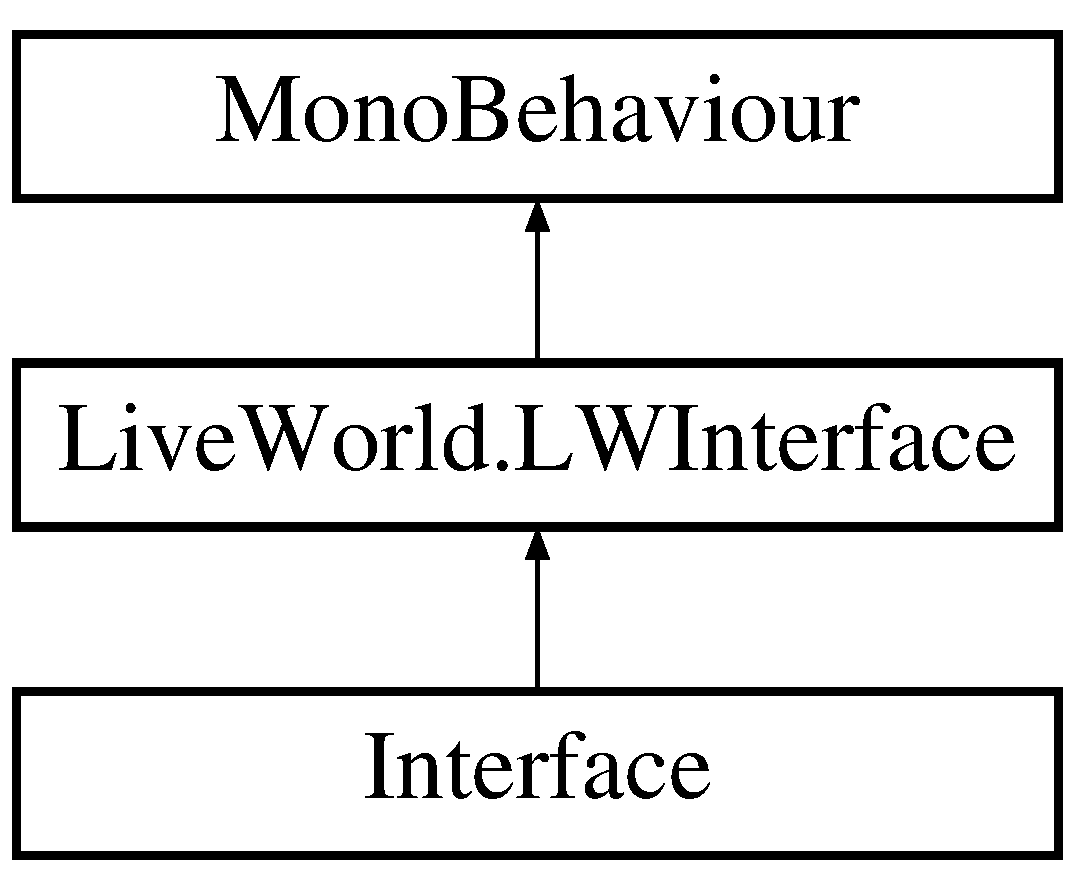
\includegraphics[height=2.000000cm]{class_interface}
\end{center}
\end{figure}
\subsection*{Public Attributes}
\begin{DoxyCompactItemize}
\item 
\hypertarget{class_interface_aef5223ae4a813051a04a201cb2b4dacb}{}string {\bfseries ip\+Address}\label{class_interface_aef5223ae4a813051a04a201cb2b4dacb}

\end{DoxyCompactItemize}


The documentation for this class was generated from the following file\+:\begin{DoxyCompactItemize}
\item 
Interface.\+cs\end{DoxyCompactItemize}

\hypertarget{class_live_world_1_1_l_w_client_method}{}\section{Live\+World.\+L\+W\+Client\+Method Class Reference}
\label{class_live_world_1_1_l_w_client_method}\index{Live\+World.\+L\+W\+Client\+Method@{Live\+World.\+L\+W\+Client\+Method}}
\subsection*{Static Public Member Functions}
\begin{DoxyCompactItemize}
\item 
\hypertarget{class_live_world_1_1_l_w_client_method_a6534e5c0c6a78fa1911d0b04814d0d69}{}static void {\bfseries Connect\+To\+Server} (string ip\+Address, int port, string password, bool use\+Password)\label{class_live_world_1_1_l_w_client_method_a6534e5c0c6a78fa1911d0b04814d0d69}

\end{DoxyCompactItemize}


The documentation for this class was generated from the following file\+:\begin{DoxyCompactItemize}
\item 
Live\+World.\+cs\end{DoxyCompactItemize}

\hypertarget{class_live_world_1_1_l_w_interface}{}\section{Live\+World.\+L\+W\+Interface Class Reference}
\label{class_live_world_1_1_l_w_interface}\index{Live\+World.\+L\+W\+Interface@{Live\+World.\+L\+W\+Interface}}
Inheritance diagram for Live\+World.\+L\+W\+Interface\+:\begin{figure}[H]
\begin{center}
\leavevmode
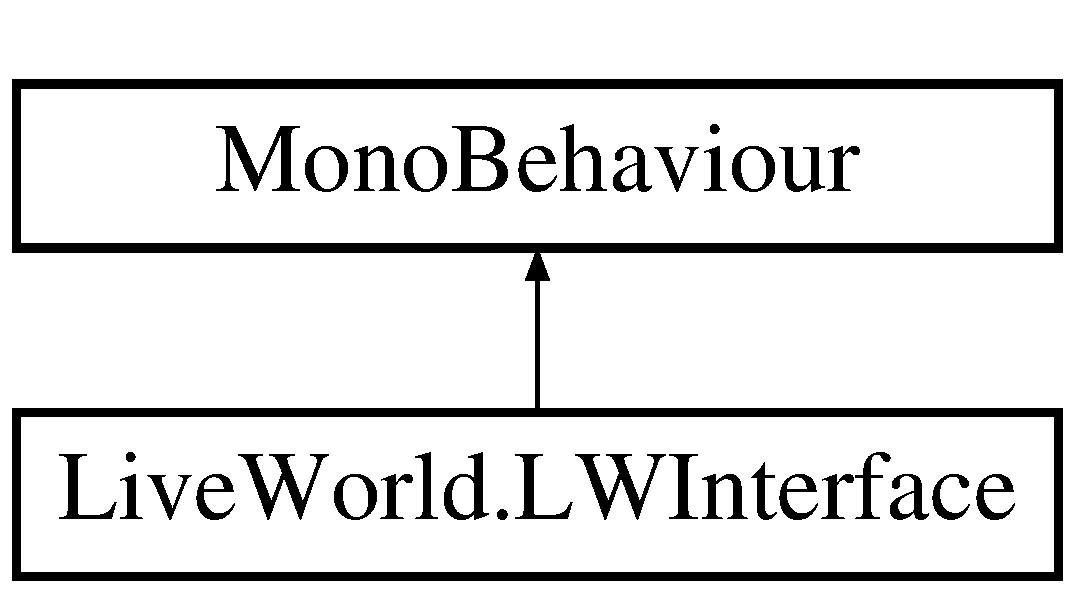
\includegraphics[height=3.000000cm]{class_live_world_1_1_l_w_interface}
\end{center}
\end{figure}
\subsection*{Classes}
\begin{DoxyCompactItemize}
\item 
class \hyperlink{class_live_world_1_1_l_w_interface_1_1_home_bar}{Home\+Bar}
\item 
class \hyperlink{class_live_world_1_1_l_w_interface_1_1_notification}{Notification}
\end{DoxyCompactItemize}
\subsection*{Static Public Member Functions}
\begin{DoxyCompactItemize}
\item 
\hypertarget{class_live_world_1_1_l_w_interface_a8689c4fab2a09c5d408e395ef92514ac}{}static void {\bfseries New\+Notification} (string Text, Notification.\+Notification\+Type Type)\label{class_live_world_1_1_l_w_interface_a8689c4fab2a09c5d408e395ef92514ac}

\end{DoxyCompactItemize}
\subsection*{Static Public Attributes}
\begin{DoxyCompactItemize}
\item 
\hypertarget{class_live_world_1_1_l_w_interface_a38a2ba545f99f8237cd0059c5403e87c}{}static bool {\bfseries show\+Home\+Bar} = false\label{class_live_world_1_1_l_w_interface_a38a2ba545f99f8237cd0059c5403e87c}

\end{DoxyCompactItemize}


The documentation for this class was generated from the following file\+:\begin{DoxyCompactItemize}
\item 
Live\+World.\+cs\end{DoxyCompactItemize}

\hypertarget{class_l_w_notification_object}{}\section{L\+W\+Notification\+Object Class Reference}
\label{class_l_w_notification_object}\index{L\+W\+Notification\+Object@{L\+W\+Notification\+Object}}
Inheritance diagram for L\+W\+Notification\+Object\+:\begin{figure}[H]
\begin{center}
\leavevmode
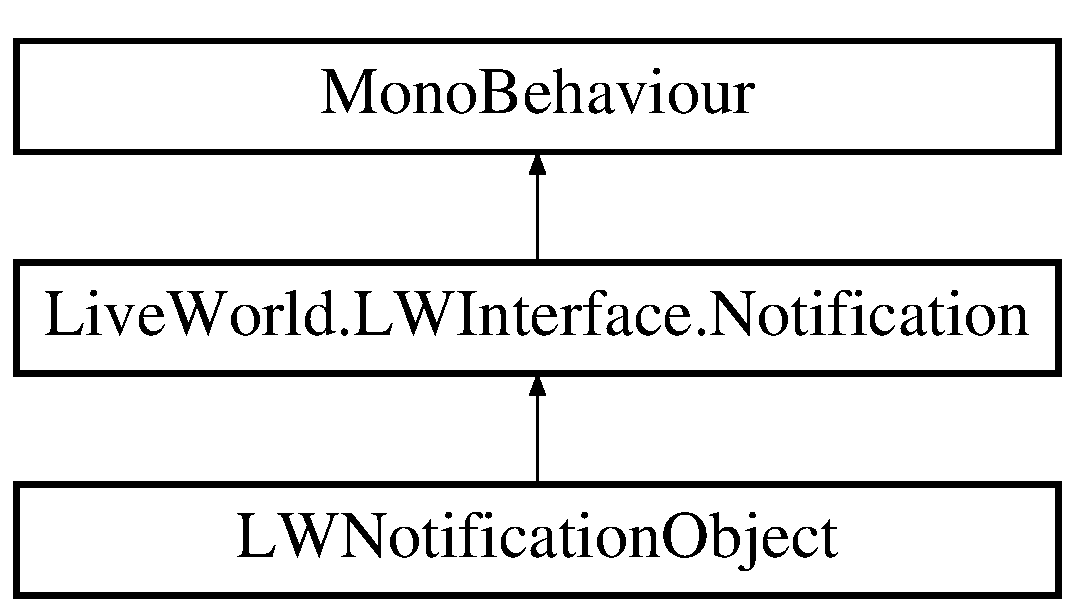
\includegraphics[height=3.000000cm]{class_l_w_notification_object}
\end{center}
\end{figure}
\subsection*{Additional Inherited Members}


The documentation for this class was generated from the following file\+:\begin{DoxyCompactItemize}
\item 
L\+W\+Notification\+Object.\+cs\end{DoxyCompactItemize}

\hypertarget{class_live_world_1_1_l_w_server_method}{}\section{Live\+World.\+L\+W\+Server\+Method Class Reference}
\label{class_live_world_1_1_l_w_server_method}\index{Live\+World.\+L\+W\+Server\+Method@{Live\+World.\+L\+W\+Server\+Method}}
\subsection*{Static Public Member Functions}
\begin{DoxyCompactItemize}
\item 
\hypertarget{class_live_world_1_1_l_w_server_method_abcdc3a1af4761172fea9ce0e8cd7a3e4}{}static void {\bfseries Initialize\+Server} (int port, int limit, string password, bool use\+Password, bool use\+N\+A\+T)\label{class_live_world_1_1_l_w_server_method_abcdc3a1af4761172fea9ce0e8cd7a3e4}

\end{DoxyCompactItemize}


The documentation for this class was generated from the following file\+:\begin{DoxyCompactItemize}
\item 
Live\+World.\+cs\end{DoxyCompactItemize}

\hypertarget{class_live_world_1_1_l_w_test_functions}{}\section{Live\+World.\+L\+W\+Test\+Functions Class Reference}
\label{class_live_world_1_1_l_w_test_functions}\index{Live\+World.\+L\+W\+Test\+Functions@{Live\+World.\+L\+W\+Test\+Functions}}
Inheritance diagram for Live\+World.\+L\+W\+Test\+Functions\+:\begin{figure}[H]
\begin{center}
\leavevmode
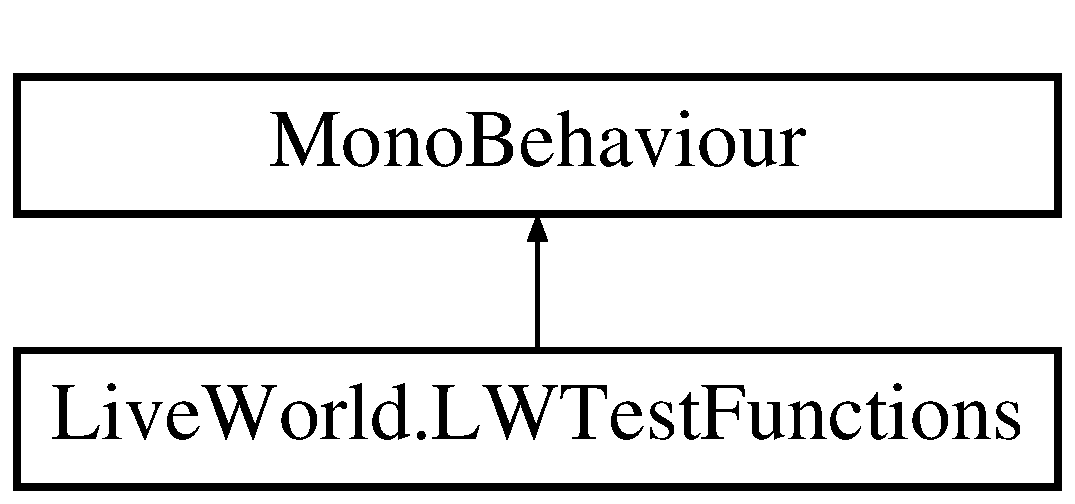
\includegraphics[height=2.000000cm]{class_live_world_1_1_l_w_test_functions}
\end{center}
\end{figure}
\subsection*{Static Public Member Functions}
\begin{DoxyCompactItemize}
\item 
\hypertarget{class_live_world_1_1_l_w_test_functions_ab54a19ea3f439ff02276719c836ce9a3}{}static void {\bfseries test} ()\label{class_live_world_1_1_l_w_test_functions_ab54a19ea3f439ff02276719c836ce9a3}

\end{DoxyCompactItemize}


The documentation for this class was generated from the following file\+:\begin{DoxyCompactItemize}
\item 
Live\+World.\+cs\end{DoxyCompactItemize}

\hypertarget{class_live_world_1_1_l_w_interface_1_1_notification}{}\section{Live\+World.\+L\+W\+Interface.\+Notification Class Reference}
\label{class_live_world_1_1_l_w_interface_1_1_notification}\index{Live\+World.\+L\+W\+Interface.\+Notification@{Live\+World.\+L\+W\+Interface.\+Notification}}
Inheritance diagram for Live\+World.\+L\+W\+Interface.\+Notification\+:\begin{figure}[H]
\begin{center}
\leavevmode
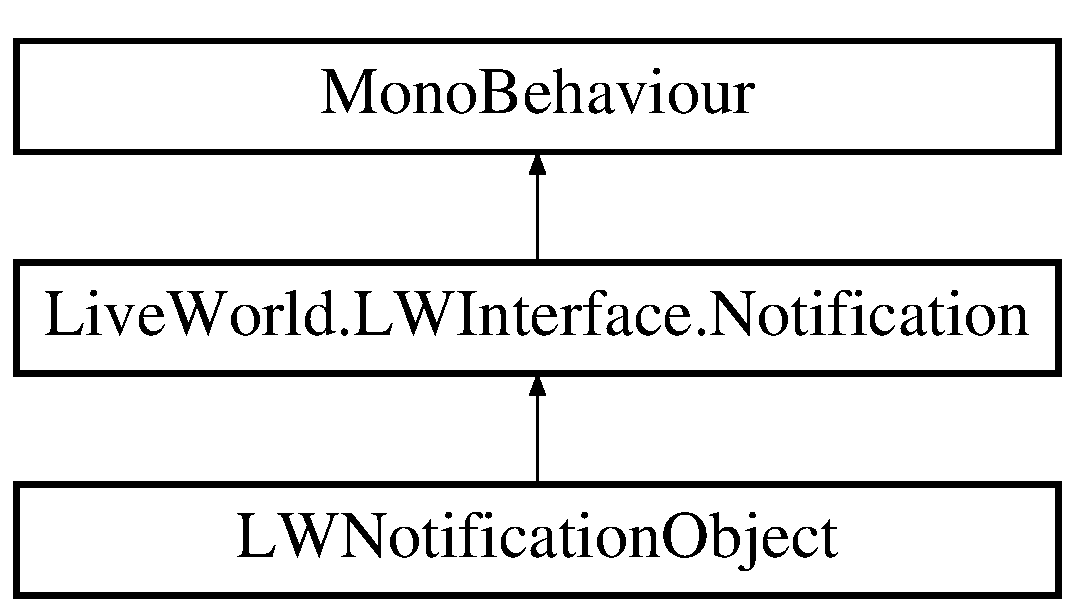
\includegraphics[height=3.000000cm]{class_live_world_1_1_l_w_interface_1_1_notification}
\end{center}
\end{figure}
\subsection*{Public Types}
\begin{DoxyCompactItemize}
\item 
\hypertarget{class_live_world_1_1_l_w_interface_1_1_notification_a136480449dfc5b6cd780c4e73c5a6e8a}{}enum {\bfseries Notification\+Type} \{ {\bfseries message}, 
{\bfseries warning}, 
{\bfseries error}
 \}\label{class_live_world_1_1_l_w_interface_1_1_notification_a136480449dfc5b6cd780c4e73c5a6e8a}

\end{DoxyCompactItemize}
\subsection*{Public Attributes}
\begin{DoxyCompactItemize}
\item 
\hypertarget{class_live_world_1_1_l_w_interface_1_1_notification_a3cb9be7169345c370db00aec68a203f2}{}string {\bfseries Text}\label{class_live_world_1_1_l_w_interface_1_1_notification_a3cb9be7169345c370db00aec68a203f2}

\item 
\hypertarget{class_live_world_1_1_l_w_interface_1_1_notification_a0718f7519e0db432e92e4112612d6df3}{}float {\bfseries Duration} = 5\label{class_live_world_1_1_l_w_interface_1_1_notification_a0718f7519e0db432e92e4112612d6df3}

\item 
\hypertarget{class_live_world_1_1_l_w_interface_1_1_notification_a25bac4d729f8b53a5fd326eaea799eac}{}float {\bfseries wanted\+X}\label{class_live_world_1_1_l_w_interface_1_1_notification_a25bac4d729f8b53a5fd326eaea799eac}

\item 
\hypertarget{class_live_world_1_1_l_w_interface_1_1_notification_a1bae44fd4d2e6f473e5679e2b6285210}{}float {\bfseries wanted\+Y}\label{class_live_world_1_1_l_w_interface_1_1_notification_a1bae44fd4d2e6f473e5679e2b6285210}

\item 
\hypertarget{class_live_world_1_1_l_w_interface_1_1_notification_adf0d8c772fe25aa51e4c91dc0a858120}{}Notification\+Type {\bfseries Type}\label{class_live_world_1_1_l_w_interface_1_1_notification_adf0d8c772fe25aa51e4c91dc0a858120}

\end{DoxyCompactItemize}


The documentation for this class was generated from the following file\+:\begin{DoxyCompactItemize}
\item 
Live\+World.\+cs\end{DoxyCompactItemize}

\hypertarget{classtest_script}{}\section{test\+Script Class Reference}
\label{classtest_script}\index{test\+Script@{test\+Script}}
Inheritance diagram for test\+Script\+:\begin{figure}[H]
\begin{center}
\leavevmode
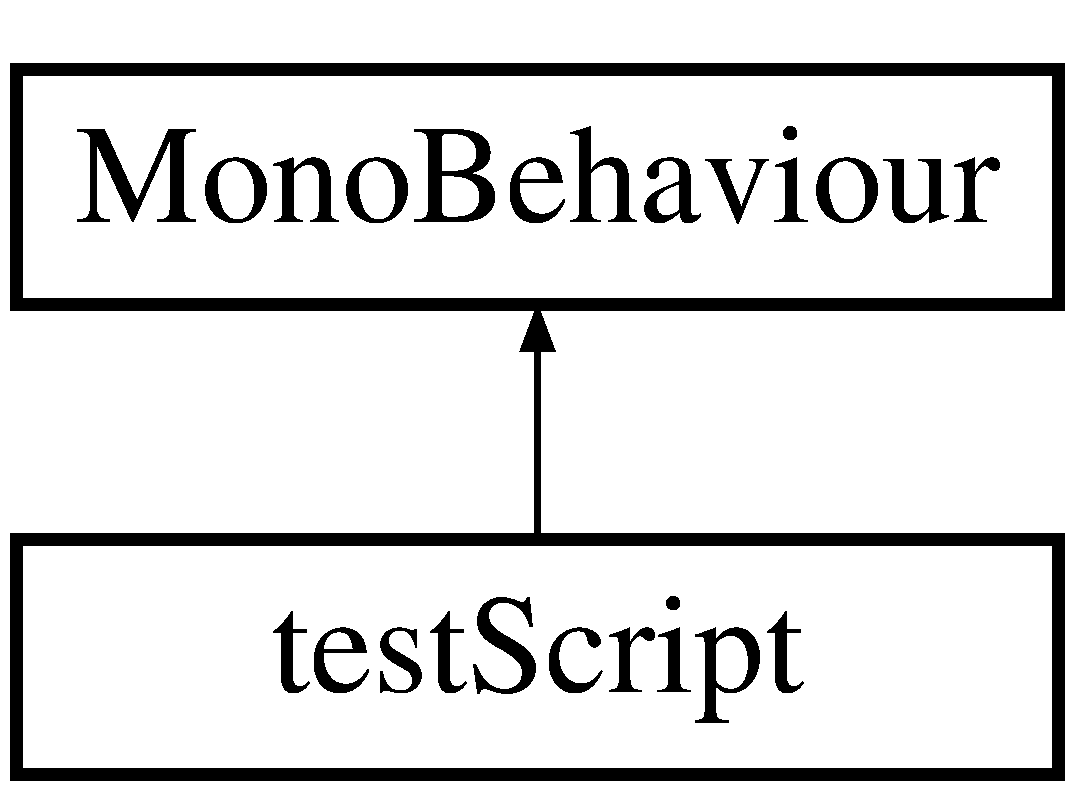
\includegraphics[height=2.000000cm]{classtest_script}
\end{center}
\end{figure}
\subsection*{Public Attributes}
\begin{DoxyCompactItemize}
\item 
\hypertarget{classtest_script_a87ee594bfc325ad5f1029d26418a6e59}{}\hyperlink{class_live_world_1_1_l_w_interface_1_1_notification}{L\+W\+Interface.\+Notification} {\bfseries new\+Notification}\label{classtest_script_a87ee594bfc325ad5f1029d26418a6e59}

\end{DoxyCompactItemize}


The documentation for this class was generated from the following file\+:\begin{DoxyCompactItemize}
\item 
test\+Script.\+cs\end{DoxyCompactItemize}

%--- End generated contents ---

% Index
\backmatter
\newpage
\phantomsection
\clearemptydoublepage
\addcontentsline{toc}{chapter}{Index}
\printindex

\end{document}
